\documentclass[10pt,reqno,a4paper,openany]{amsbook}
\usepackage{etex}
\usepackage[utf8]{inputenc}
\usepackage[english]{babel}
\usepackage{etoolbox,chngcntr}
\usepackage{amsmath,amsthm,amssymb,array,stmaryrd,color,graphicx,mathtools,multirow,setspace}
\usepackage{soul}\setul{0.3ex}{}
\usepackage{bussproofs}
\usepackage{manfnt}
\usepackage{xspace}
\usepackage{longtable}
\usepackage{booktabs}
\usepackage[protrusion=true,expansion=true]{microtype}
\usepackage[bookmarksdepth=2,pdfencoding=auto]{hyperref}

\graphicspath{{images/}}
\usepackage{libertine}

% Hack to load extpfeil from https://tex.stackexchange.com/a/297109/32372
\expandafter\def\csname opt@stmaryrd.sty\endcsname
{only,shortleftarrow,shortrightarrow}
\usepackage{extpfeil}
\newextarrow{\xbigtoto}{{20}{20}{20}{20}}
   {\bigRelbar\bigRelbar{\bigtwoarrowsleft\rightarrow\rightarrow}}

\usepackage[all]{xy}
\usepackage{tikz}
\usetikzlibrary{calc,shapes.callouts,shapes.arrows,matrix,patterns}
\newcommand{\hcancel}[5]{%
    \tikz[baseline=(tocancel.base)]{
        \node[inner sep=0pt,outer sep=0pt] (tocancel) {#1};
        \draw[red, line width=0.3mm] ($(tocancel.south west)+(#2,#3)$) -- ($(tocancel.north east)+(#4,#5)$);
    }%
}

\usepackage[natbib=true,style=numeric,maxnames=10]{biblatex}
\usepackage[babel]{csquotes}
\bibliography{algar-lecture-notes}

\theoremstyle{definition}
\newtheorem{defn}{Definition}[chapter]
\newtheorem{ex}[defn]{Example}

\theoremstyle{plain}
\newtheorem{prop}[defn]{Proposition}
\newtheorem{cor}[defn]{Corollary}
\newtheorem{lemma}[defn]{Lemma}
\newtheorem{thm}[defn]{Theorem}
\newtheorem{scholium}[defn]{Scholium}

\theoremstyle{remark}
\newtheorem{rem}[defn]{Remark}
\newtheorem{question}[defn]{Question}
\newtheorem{speculation}[defn]{Speculation}
\newtheorem{caveat}[defn]{Caveat}
\newtheorem{conjecture}[defn]{Conjecture}

\newcommand{\ZZ}{\mathbb{Z}}
\newcommand{\FF}{\mathbb{F}}
\renewcommand{\AA}{\mathbb{A}}
\newcommand{\A}{\mathcal{A}}
\newcommand{\B}{\mathcal{B}}
\newcommand{\C}{\mathcal{C}}
\newcommand{\D}{\mathcal{D}}
\newcommand{\E}{\mathcal{E}}
\newcommand{\F}{\mathcal{F}}
\newcommand{\G}{\mathcal{G}}
\let\acuteH\H
\newcommand{\konig}{K\acuteH onig}
\renewcommand{\H}{\mathcal{H}}
\renewcommand{\O}{\mathcal{O}}
\newcommand{\K}{\mathcal{K}}
\newcommand{\N}{\mathcal{N}}
\newcommand{\M}{\mathcal{M}}
\renewcommand{\L}{\mathcal{L}}
\renewcommand{\P}{\mathcal{P}}
\newcommand{\R}{\mathcal{R}}
\newcommand{\T}{\mathcal{T}}
\newcommand{\I}{\mathcal{I}}
\newcommand{\J}{\mathcal{J}}
\renewcommand{\S}{\mathcal{S}}
\newcommand{\U}{\mathcal{U}}
\newcommand{\V}{\mathcal{V}}
\newcommand{\NN}{\mathbb{N}}
\newcommand{\PP}{\mathbb{P}}
\newcommand{\RR}{\mathbb{R}}
\newcommand{\CC}{\mathbb{C}}
\newcommand{\QQ}{\mathbb{Q}}
\newcommand{\GG}{\mathbb{G}}
\newcommand{\TT}{\mathbb{T}}
\newcommand{\aaa}{\mathfrak{a}}
\newcommand{\bbb}{\mathfrak{b}}
\newcommand{\ccc}{\mathfrak{c}}
\newcommand{\ppp}{\mathfrak{p}}
\newcommand{\qqq}{\mathfrak{q}}
\newcommand{\mmm}{\mathfrak{m}}
\newcommand{\nnn}{\mathfrak{n}}
\newcommand{\?}{\,{:}\,}
\renewcommand{\_}{\mathpunct{.}\,}

\newenvironment{indentblock}{%
  \list{}{\leftmargin\leftmargin}%
  \item\relax
}{%
  \endlist
}

\newcommand{\defeq}{\vcentcolon=}
\newcommand{\defequiv}{\vcentcolon\equiv}
\newcommand{\seq}[1]{\mathrel{\vdash\!\!\!_{#1}}}

\definecolor{gray}{rgb}{0.7,0.7,0.7}

\title{The curious world of constructive mathematics}
\author{Ingo Blechschmidt \vspace*{-2em}}
%\email{iblech@speicherleck.de}

\makeatletter
\counterwithout{section}{chapter}
\counterwithout{footnote}{chapter}
\counterwithout{table}{chapter}
\counterwithout{figure}{chapter}
\patchcmd{\@thm}{\let\thm@indent\indent}{\let\thm@indent\noindent}{}{}
\patchcmd{\@thm}{\thm@headfont{\scshape}}{\thm@headfont{\bfseries}}{}{}
\patchcmd{\@makechapterhead}{\chaptername}{Lecture}{}{}
\patchcmd{\@chapter}{\chaptername}{Part}{}{}
\patchcmd{\@schapter}{\chaptername}{Part}{}{}
\addto\captionsenglish{\renewcommand\chaptername{Lecture}}
\def\l@section{\@tocline{1}{0pt}{1pc}{}{}} % \bfseries}}
\def\l@chapter{\@tocline{-1}{12pt}{0pt}{}{\bfseries}}
\renewcommand\thechapter{\Roman{chapter}}
\newcommand{\nocontentsline}[3]{}
\newcommand{\tocless}[1]{\let\addcontentsline=\nocontentsline}
\normalparindent=12pt
\parindent=\normalparindent
\renewenvironment{proof}[1][\proofname]{\par
  \pushQED{\qed}%
  \normalfont \topsep6\p@\@plus6\p@\relax
  \trivlist
  \item[\hskip\labelsep
        \itshape
    #1\@addpunct{.}]\ignorespaces
}{%
  \popQED\endtrivlist\@endpefalse
}
\let\@afterindenttrue\@afterindentfalse
\def\subsection{\@startsection{subsection}{2}%
  {0pt}{.5\linespacing\@plus.7\linespacing}{-.5em}%
  {\normalfont\bfseries}}
\makeatother

\newenvironment{intro}{\begin{quote}}{\end{quote}\bigskip}

\newtheorem{exercise}[defn]{Exercise}
\renewcommand{\theenumi}{\alph{enumi}}

\urlstyle{sf}

\newcommand{\cl}{\mathrm{cl}}
\newcommand{\notnot}{\emph{not~not}}

\begin{document}

\begin{abstract}
Constructive mathematics is a flavor of mathematics in which we use the
axiom of choice and the technique of proof by contradiction only in
certain special cases. The square root of two is constructively still
irrational, but there might be vector spaces without a basis.

As a result, proofs are more informative (for instance regarding
bounds), finer distinctions can be made (for instance between positive
existence and mere impossibility of non-existence) and results apply
more generally: Every constructive result also has a geometric
interpretation, where it applies to continuous families, and an
algorithmic interpretation, yielding computational witnesses such as
procedures for computing the objects whose existence has been shown.

Relinquishing the axiom of choice and the principle of excluded middle also
allows us to explore axioms and notions which are incompatible with
these classical laws, such as mathematical settings in which all
functions are continuous or in which the intuitive idea of a ``generic
ring'' can be put on a firm basis.
\end{abstract}

{
\renewcommand{\newpage}{\ }
\renewcommand{\vfill}{\ }
\renewcommand{\vfil}{\ }
\enlargethispage{7em}
{\vspace*{-6em}\centering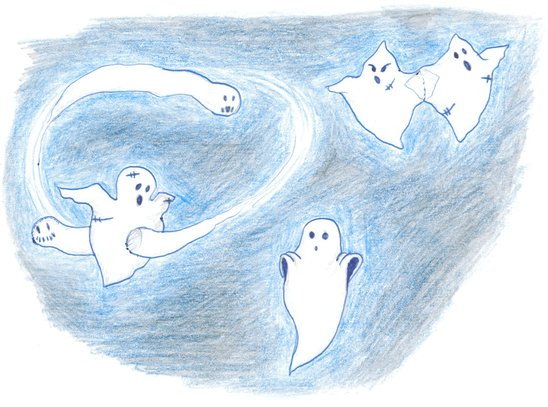
\includegraphics[width=0.3\textwidth]{phantoms}\par}
\maketitle
}

\setcounter{tocdepth}{1}
{
\renewcommand{\newpage}{\ }
\tableofcontents
}
\thispagestyle{empty}


\chapter{A first glimpse of constructive mathematics}

\begin{intro}
\it
This lecture provides a first glimpse of constructive mathematics with a
focus on applications of constructive mathematics and on providing
intuition for quickly discerning which techniques and results hold
constructively.

This account is an update and translation of~\cite[Section~1]{blechschmidt:pizzaseminar}
and references
include~\cite{bauer:five-stages-video,bauer:five-stages-article,avigad:constructive,sep:intuitionistic-logic,dummett:basis,melikhov:intuitionistic-logic,streicher:constructive}
or more
specifically~\cite{mines-richman-ruitenburg:constructive-algebra,lombardi-quitte:constructive-algebra}
for constructive algebra and~\cite{bishop-bridges:bible} for constructive
analysis.
\end{intro}

\begin{prop}There are irrational numbers~$x$ and~$y$ such that~$x^y$ is
rational.
\end{prop}
\begin{proof}[First proof] The number~$\sqrt{2}^{\sqrt{2}}$ is rational or
irrational. In the first case, set~$x \defeq \sqrt{2}$, $y \defeq \sqrt{2}$.
In the second case, set~$x \defeq \sqrt{2}^{\sqrt{2}}$, $y \defeq \sqrt{2}$.
\end{proof}
\begin{proof}[Second proof] Set~$x \defeq \sqrt{2}$ and~$y \defeq \log_{\sqrt{2}} 3$.
Then~$x^y = 3$ is rational. The verification that~$y$ is irrational is even
easier than that of~$\sqrt{2}$.\footnote{Let~$y = a/b$ with~$a, b \in \ZZ$
and~$b \neq 0$. Since~$y > 0$, we may assume~$a, b \in \NN$. Then~$3 =
(\sqrt{2})^{a/b}$, hence~$3^{2b} = 2^a$. This is in contradiction to the
uniqueness of the prime factor decomposition, since the factor~$3$ occurs on
the left but not on the right.}
\end{proof}

The first proof is \emph{unconstructive}: It does not actually give us an
example for a pair~$(x,y)$ as desired. In contrast, the second proof is
constructive -- the existential claim is verified by an explicit construction
of a suitable example.

Of the many axioms and inference rules of classical logic, exactly one is
responsible for enabling unconstructive arguments, namely the \emph{principle
of excluded middle}:
\[ \varphi \ \vee\ \neg\varphi. \]
The first proof above used this principle in its very first step. In
constructive mathematics, we abstain from this principle; we build
constructive mathematics on \emph{intuitionistic logic}, which contains neither
this principle nor the (equivalent) \emph{principle of double negation
elimination} stating~$\neg\neg\varphi \Rightarrow \varphi$, and insofar as we
layer a set theory on top of our logical foundation, we abstain from the axiom
of choice (which in presence of other common set-theoretical axioms implies the
principle of excluded middle, see Exercise~\ref{ex:diaconescu}) and from Zorn's lemma. As a
consequence, we cannot generally reason by contradiction in constructive
mathematics, and to demonstrate the existence of an object
it is not enough that its nonexistence would entail a contradiction.

Importantly, in constructive mathematicics we do \emph{not} claim that the principle of
excluded middle is false. \marginpar{\dbend}
Indeed, intuitionistic logic is downwardly compatible
with classical logic (every intuitionistic proof is a fortiori also a classical
proof), and some special instances of the principle of excluded middle and with
it some special instances of proof by contradiction are
intuitionistically verifiable (an example is given in
Proposition~\ref{prop:discreteness}). Instead, in constructive mathematics we
merely do not use the principle of excluded middle.

Also, deducing from a statement of the form~``$\exists x \in X\_ \varphi(x)$''
that there actually is an element~$x \in X$ such that~$\varphi(x)$, and then
using this particular element in the rest of an argument, is intuitionistically a
valid logical inference, just as it is in classical logic. The axiom of choice
is unrelated to this kind of proof step, even though they are sometimes
mistaken.


\section{Proof by contradiction vs. proof of a negation}

A rumor about constructive mathematics states that constructively, the term
``contradiction'' would be generally forbidden. This rumor is false. In fact, we need
to distinguish between two distinct figures of proof which are often conflated
in classical informal mathematics:

\begin{enumerate}
\item[1.] ``Assume~$\neg\varphi$. Then $\ldots$, a contradiction.
Hence~$\neg\varphi$ was false and thus~$\varphi$ holds.''
\item[2.] ``Assume~$\psi$. Then $\ldots$, a contradiction. Hence~$\neg\psi$.''
\end{enumerate}

Arguments of the first form are proper proofs by contradiction and hence not
generally accepted in constructive mathematics. What they establish is
only~$\neg(\neg\varphi)$, the impossibility of~$\neg\varphi$; constructively,
this is weaker than a positive affirmation of~$\varphi$. Though there are
situations in which~$\neg\neg\varphi$ implies~$\varphi$, generally it does not
and hence intuitionistically arguments of the first form fail to
estabilish~$\varphi$.

In contrast, arguments of the second kind are fine from an intuitionistic point
of view: They do not constitute proper proofs by contradiction, but instead are proofs of negated
statements. That such proofs are valid follows directly from the definition of
negation as a certain
implication (which, incidentally, texts on classical logic often also adopt):
\[ \neg\psi \defequiv (\psi \Rightarrow \bot), \]
where~``$\bot$'', pronounced ``bottom'', is \emph{absurdity}, a canonical false
statement. (Informally, absurdity is also written as~``$\lightning$'' or~``$1 = 0$''.)
Hence, to establish~$\neg\psi$, we may give a proof of~$\bot$ under
the assumption~$\psi$, just as we may give a proof of~$\beta$ under the
assumption~$\alpha$ if we want to prove~$\alpha \Rightarrow \beta$.

The two proofs below of the following fact from number theory demonstrate the
difference:
\begin{prop}\label{prop:sqrt2}The number~$\sqrt{2}$ is not rational.\end{prop}
\begin{proof}[Proof (only valid classically)]
Assume that the claim is false, that is, that the number~$\sqrt{2}$ is
\emph{not not} rational. Then~$\sqrt{2}$ is rational. Hence there are
integers~$a$ and~$b$ with~$\sqrt{2} = a / b$. Thus~$2b^2 = a^2$. This identity
contradicts the uniqueness of the prime factor decomposition, since the
factor~$2$ occurs an odd number of times on the left but an even number of
times on the right.
\end{proof}
\begin{proof}[Proof (also valid intuitionistically)]
Assume that the number~$\sqrt{2}$ is rational. Then there are integers~$a$
and~$b$, \ldots, a contradiction.
[The requisite theorem on the uniqueness of the prime factor decomposition admits an
intuitionistic proof.]
\end{proof}

Constructively stronger than the statement that~$\sqrt{2}$ is merely
\emph{not rational} is the statement that for every rational number~$x$
the distance~$|\sqrt{2} - x|$ is positive. This stronger claim admits an
intuitionistic proof as well (Exercise~\ref{ex:sqrt2}).


\section{Constructive meaning of mathematical statements}

By our training in classical mathematics, abstaining from the principle of
excluded middle can feel peculiar, perhaps even outrageous: Isn't it obvious
that every mathematical statement is true or false?

This sense of bewilderment is resolved by observing that \emph{even though
constructive mathematicians use the same logical symbols, they have a slightly
different meaning in mind.} When a constructive mathematician argues for some
statement~$\varphi$, they mean that they have an \emph{explicit witness}
for~$\varphi$. This shift in meaning from the classical interpretation is
elaborated by the \emph{Brouwer--Heyting--Kolmogorov interpretation} sketched
below. It is informal and philosophical in nature and not without
issues~\cite{artemov:bhk,sanz-piecha:critical-bhk,dalen:bhk}, but still a useful guide to
the constructive meaning of mathematical statements.


\subsection{The Brouwer--Heyting--Kolmogorov interpretation}

The notion of witnesses is compositional in nature and starts out with the notion of witnesses for \emph{atomic
statements}, those not built from substatements using the logical
connectives~$\wedge,\vee,\Rightarrow$ or the quantifiers~$\forall,\exists$. For
instance, in formal number theory, the atomic statements are of the form
``$s = t$'',
where~$s$ and~$t$ are terms for natural numbers; statements of this form are so
simple that we can check them directly so that witnesses don't need to supply
particular additional information. We hence decree that true atomic statements
have trivial witnesses and that false atomic statements have no witnesses at
all.

Table~\ref{table:bhk} explains how compound statements should be witnessed. For
instance, a witness of a statement of the form
\[ \forall n \? \NN\_ \bigl(\varphi(n) \Rightarrow \psi(n)\bigr) \]
is a rule explaining how, for every natural number~$n : \NN$, witnesses
for~$\varphi(n)$ give rise to witnesses for~$\psi(n)$.

\begin{table}
  \centering
  \small
  \renewcommand{\arraystretch}{1.3}
  \begin{tabular}{@{}rp{4.3cm}p{5.3cm}@{}}
    \toprule
    & {classical logic} & {intuitionistic logic}
    \\\midrule
    statement $\varphi$ & The statement $\varphi$ holds. & We have a witness for $\varphi$. \\
    $\bot$ & A contradiction holds. & We have a witness for a contradiction. \\
    $\varphi \wedge \psi$ & $\varphi$ and $\psi$ hold. & We have a witness for~$\varphi$ and for~$\psi$. \\
    $\varphi \vee \psi$ & $\varphi$ or $\psi$ hold. & We have a witness for~$\varphi$ or for~$\psi$. \\
    $\varphi \Rightarrow \psi$ & If~$\varphi$ holds, then so does~$\psi$. &
    We can (uniformly) construct witnesses for~$\psi$ from witnesses
    for~$\varphi$. \\
    $\neg\varphi$ &
      $\varphi$ does not hold. &
      There is no witness for~$\varphi$. \\
    $\forall x\?X\_ \varphi(x)$ & For all $x \? X$ it holds that~$\varphi(x).$ &
      We can (uniformly) construct, for all~$x \? X$, witnesses for~$\varphi(x)$. \\
    $\exists x\?X\_ \varphi(x)$ & \raggedright There is at least one~$x \? X$
    such that~$\varphi(x)$ holds. & {\raggedright
      We have a~$x \? X$ together with a witness for~$\varphi(x)$.} \\
    \bottomrule
  \end{tabular}
  \caption{\label{table:bhk}Informal recursive definition of the notion of witnesses.}
\end{table}

\begin{ex}
According to the Brouwer--Heyting--Kolmogorov interpretation, the principle of
excluded middle states that we can construct, for every~$\varphi$,
either a witness for~$\varphi$ or a witness for~$\neg\varphi$. This claim is
obviously false.
\end{ex}

\begin{ex}
The BHK interpretation of a doubly negated statement~$\neg\neg\varphi$ is that
there is no witness for~$\neg\varphi$. This state of affairs does not entail
that we actually have a witness for~$\varphi$; in a sense, the
statement~$\varphi$ is only ``potentially true''.
\end{ex}

\begin{ex}
Assuming that we cannot find our apartment key, but know that it has to be
somewhere (because we used it last night to unlock the door), constructively we
can only defend the doubly negated statement
\[ \neg\neg (\exists x\_ \text{the key is at position~$x$}). \]
\end{ex}

\begin{ex}
We are running errands and are remembering that we need to fetch certain
ingredients. Unfortunately we don't recall any of them right now. Then we can
constructively defend the statement that the set of ingredients to fetch is not
empty, not however the stronger statement that this set is inhabited.
\end{ex}

\begin{ex}[\cite{sigfpe:katemoss,bbc:katemoss}]
A video surfaced depicting Kate Moss taking drugs, more precisely either drugs
of some type~A or drugs of some type~B. However from the video it wasn't clear
which type of drug it actually was. Hence there was no evidence for either type
of consumption; Kate Moss wasn't prosecuted.
\end{ex}

\begin{rem}The reference of an unspecified ``we'' in table~\ref{table:bhk}
renders our account of the BHK interpretation not only informal, but is also
somewhat misleading. As in classical mathematics, judgments of intuitionistic
logic do not actually depend on you, me or other mathematicians. It's perfectly
possible that statements which haven't yet been constructively verified admit
(as yet unknown) witnesses. More details can be found
in~\cite[pp.~42]{kohlenbach:applprooftheory} and
in~\cite{artemov:bhk,sanz-piecha:critical-bhk,dalen:bhk}. The
Brouwer--Heyting--Kolmogorov interpretation is made more formal and precise by
\emph{realizability theory}~\cite{bauer:realizability,oosten:realizability}.
\end{rem}


\subsection{The computability interpretation}

A second interpretation of mathematical statements suited for constructive
mathematics is given by the following motto: In a certain sense, \emph{we
accept a mathematical statement in constructive mathematics if and only if
there is a computer program witnessing it in finite time.} For instance, that
the statement
\[ \forall n \? \NN\_ \exists p \? \NN\_ p \geq n \wedge \text{$p$ is prime} \]
is valid in constructive mathematics corresponds to the fact that there is a
computer program which reads a number~$n$ as input and then, after some
computation, produces a prime number~$p \geq n$ as output (together with a
witness that~$p$ is in fact greater or equal than~$n$ and that~$p$ is prime).

For the motto to be correct, the notion of ``witnessed by a computer program''
has to be interpreted in sufficiently generous manner, not least because
uncountable and uncomputable structures have their place in constructive
mathematics just as in classical mathematics. A more formal rendition is
provided by the celebrated \emph{Curry--Howard correspondence} and
\emph{propositions as (some) types}.


\subsection{The geometric interpretation}

A third interpretation of mathematical statements suited for constructive
mathematics, and of a substantially different kind than the BHK and the
computability interpretation, is provided by geometry. In a certain sense,
\emph{we accept a mathematical statement in constructive mathematics if and
only if it holds locally in continuous families}.

For instance, while it is a fact of classical mathematics that every complex
number has a square root, a fundamental observation in complex analysis is that
such roots cannot be picked in a locally continuous manner. Hence the standard
formulation of the fundamental theorem of algebra fails in constructive
mathematics.\footnote{More precisely, the fundamental theorem of algebra fails
for the complex numbers built from pairs of Dedekind reals. Constructively, the
reals built using Dedekind cuts are not the same as the reals built using
Cauchy sequences; in fact, the latter are a subset of the former and serve a
different purpose. Such a bifurcation of classically equivalent notions is
typical of constructive mathematics. The fundamental theorem of algebra is
correct for the flavor of complex numbers built from Cauchy
reals~\cite{ruitenburg:roots}, and also for the algebraic
numbers~\cite[Section~VII.4]{mines-richman-ruitenburg:constructive-algebra}
[XXX insert better references] and for complex polynomials (of either flavor)
which are separable. Furthermore, the fundamental theorem of algebra holds in
an approximate sense and in a multiset sense~\cite{richman:fta}, and the
standard version only requires mild choice
principles~\cite{bridges-richman-schuster:wcc}.} This example will be discussed
in more detail in Section~\ref{sect:fta}.

The geometric interpretation not only gives transparent explanations to the
logical subtleties of constructive mathematics, but is in a more precise form
also the workhorse of many modern applications of constructive mathematics to
mathematics in general. We will hence dedicate ample of space to the geometric
interpretation by devoting Lecture~\ref{lect:toposes} to it, and will discuss
some of its more advanced applications in Lecture~\ref{lect:generic}.


\section{Finer distinctions supported by constructive mathematics}


\section{Exercises}

\begin{exercise}[Constructive status of classical tautologies]\label{ex:tautologies}
Which of the following classical tautologies can reasonably be expected to
admit constructive proofs?
\begin{enumerate}
\item $\neg(\alpha \vee \beta) \ \Longrightarrow\ \neg\alpha \wedge \neg\beta$
\item $\neg(\alpha \wedge \beta) \ \Longrightarrow\ \neg\alpha \vee \neg\beta$
\item $(\alpha \Rightarrow \beta) \ \Longrightarrow\ (\neg\alpha \vee \beta)$
\item $(\alpha \vee \beta) \wedge \neg\alpha \ \Longrightarrow\ \beta$
\item $\forall M\?P(X)\_ (\exists x\?X\_ x \in M) \vee M = \emptyset$
(already interesting for~$X = \{\star\}$)
\item $\forall n\?\NN\_ (n = 0 \vee n \neq 0)$
\item $\forall x\?\RR\_ (x = 0 \vee x \neq 0)$
\item $\forall x\?\RR\_ (\neg(\exists y\?\RR\_ xy=1) \Rightarrow x = 0)$
\item $\forall z\?\overline{\QQ}\_ (z = 0 \vee z \neq 0)$
\item $\forall f \? \NN \to \{0,1\}\_ (\neg\neg\exists n \? \NN\_ f(n) = 0)
\Rightarrow (\exists n \? \NN\_ f(n) = 0)$ (Markov's principle)
\item $\forall f \? \NN \to \{0,1\}\_ \exists n \? \NN\_ (f(n) = 1
\Rightarrow (\forall m \? \NN\_ f(m) = 1))$ (Drinker's paradox)
\item $\forall f \? \NN \to \{0,1\}\_ (\exists n \? \NN\_ f(n) = 0) \vee
(\forall n \? \NN\_ f(n) = 1)$
\item $\forall f \? \NN_\infty \to \{0,1\}\_ (\exists n \? \NN_\infty\_ f(n) = 0) \vee
(\forall n \? \NN_\infty\_ f(n) = 1)$

{\noindent\scriptsize\emph{Remark.} The set~$\NN_\infty$ is the \emph{one-point
compactification} of~$\NN$. A sensible definition of it in constructive mathematics
is as the set of decreasing binary sequences~$(x_0,x_1,x_2,\ldots)$. The
naturals embed into~$\NN_\infty$ by mapping~$n$ to the sequence~$1^n 0^\omega =
(1,\ldots,1,0,\ldots,0)$, and an element not in the image of this embedding
is~$\infty \defeq 1^\omega = (1,1,\ldots)$. Assuming the principle of excluded
middle (or already weaker principles), every element of~$\NN_\infty$ is of one
of these two forms. Martín Escardó has worked extensively on unexpected
instances of the principle of omniscience for searchable sets
like~$\NN_\infty$~\cite{escardo:omniscience1,escardo:omniscience2,escardo:omniscience}.\par}
\end{enumerate}
\end{exercise}

\begin{exercise}[Basics on negation]
Recalling that negation is defined as implying absurdity,~$\neg\varphi
\defequiv (\varphi \Rightarrow \bot)$, verify intuitionistically without
recourse to truth tables:
\begin{enumerate}
\item $\varphi \Rightarrow \neg\neg\varphi$
\item $\neg\neg\neg\varphi \Leftrightarrow \neg\varphi$
\item $\neg\neg(\varphi \vee \neg\varphi)$
\item $\neg\neg(\alpha \wedge \beta) \Leftrightarrow (\neg\neg\alpha \wedge
\neg\neg\beta)$
\item $\neg(\alpha \vee \beta) \Longleftrightarrow (\neg\alpha \wedge \neg\beta)$
\item $(\neg\neg\alpha \wedge (\alpha \Rightarrow \neg\neg\beta)) \Longrightarrow
\neg\neg\beta$
\item $(\forall\psi\_ (\psi \vee \neg\psi))
\Longleftrightarrow (\forall\psi\_ ((\neg\neg\psi) \Rightarrow
\psi))$

{\noindent\scriptsize\emph{Hint.}
Don't try to verify that double negation elimination for a specific
statement~$\psi$ implies the principle of excluded middle for that same
statement~$\psi$ -- this cannot be shown. There are subtleties regarding the
quantification over $\psi$ (this is not expressible in pure first-order logic),
however the exercise is still instructive if we gloss over this issue.\par}
\end{enumerate}
\end{exercise}

\begin{exercise}[An epistemic riddle on transcendental numbers]
Verify, using a proof by contradiction, that at least one of the numbers~$e +
\pi$ and~$e - \pi$ is transcendental; and that at least one of the
numbers~$e + \pi$ and~$e \cdot \pi$ is transcendental.
\end{exercise}

\begin{exercise}[A stronger form of the irrationality of~$\sqrt{2}$]
\label{ex:sqrt2}
Mine the proof of Proposition~\ref{prop:sqrt2} to give an intuitionistic proof
that for every rational number~$x$, the distance~$|\sqrt{2}-x|$ is positive.

{\noindent\scriptsize\emph{Note.} Strictly speaking, this exercise presupposes
familiarity with an intuitionistic account of the basics of undergraduate real
analysis. Without it, one cannot really be expected to precisely think about
these matters. One such account (though assuming the axiom of dependent choice)
is~\cite{bishop-bridges:bible}. However, this exercise is insightful even when carried out
slightly informally. Keep in mind that, to show that a real number is positive,
constructively it is not enough to merely verify that it cannot be zero or
negative. A safe way to verify that a real number~$a$ is positive is to exhibit
a rational number~$b$ such that~$a \geq b > 0$.\par}
\end{exercise}

\begin{exercise}[Brouwerian counterexamples]
Show that each of the following statements implies the principle of excluded middle,
hence is not available in constructive mathematics.
\begin{enumerate}
\item Every ideal of~$\ZZ$ is finitely generated.

{\noindent\scriptsize\emph{Hint.} Use that finitely generated ideals of~$\ZZ$
are principal ideals and consider the ideal~$\aaa \defeq \{ x \in \ZZ
\,|\, x = 0 \vee \varphi \}$.\par}

{\noindent\scriptsize\emph{Remark.} The failure of every ideal of~$\ZZ$ to be
finitely generated should not be misconstrued to exclaim that in constructive
mathematics, there suddenly would be ideals of~$\ZZ$ of infinite rank. The
failure is simply because, given an abstract ideal, we cannot pinpoint a finite
system of generators.\par}

\item Over every field, the polynomial~$X^2 + 1$ is either reducible or
irreducible.

{\noindent\scriptsize\emph{Hint.} Consider the field~$K \defeq \{ z \in \QQ(i)
\,|\, z \in \QQ \vee \varphi \}$.\par}

\item Subsets of Kuratowski-finite sets are Kuratowski-finite.

{\noindent\scriptsize\emph{Note.} A set~$X$ is \emph{Kuratowski-finite} if and
only if, for some number~$n \in \NN$, there is a surjective map~$[n] \to X$,
where~$[n] = \{ 0,1,\ldots,n-1 \}$. More briefly, a set~$X$ is
Kuratowski-finite iff its elements can be enumerated: $X = \{x_1,\ldots,x_n \}$.\par}
\end{enumerate}
Show that the following statement implies Markov's principle (from
Exercise~\ref{ex:tautologies}):
\begin{enumerate}
\addtocounter{enumi}{3}
\item Every real number which is not zero is invertible.
\end{enumerate}
\noindent
Brouwerian counterexamples abound in constructive mathematics; when developing
a constructive account of a theory, they help to clearly demarcate its limits.
As such additional Brouwerian counterexamples can be found in most texts on
constructive mathematics, such
as~\cite{mines-richman-ruitenburg:constructive-algebra}; a compilation mainly
from constructive analysis can be found
in~\cite{mandelkern:brouwerian-counterexamples}.
\end{exercise}

\begin{exercise}[Diaconescu's theorem]
\label{ex:diaconescu}
The axiom of choice can be put as: ``Every surjective map has a
section.'' (A \emph{section}~$s$ to a surjective map~$f$ is a map in the other direction such that~$f \circ s =
\mathrm{id}$.) A theorem of Diaconescu states that
the axiom of choice implies the principle of excluded middle. To this end, let~$\varphi$ be a
statement and consider the subsets
\begin{align*}
  U &= \{ x \in X \,|\, (x = 0) \vee \varphi \} \\
  V &= \{ x \in X \,|\, (x = 1) \vee \varphi \}
\end{align*}
of the discrete set~$X \defeq \{ 0,1 \}$.
\begin{enumerate}
\item Verify that~$U = V$ if and only if~$\varphi$.
\item Using that~$x = y \vee x \neq y$ for all elements~$x,y \in X$, show that
the existence of a section of the surjective map
\[ \begin{array}{@{}rcl@{}}
  X &\longrightarrow& \{U,V\} \\
  0 &\longmapsto& U \\
  1 &\longmapsto& V
\end{array} \]
implies~$\varphi \vee \neg\varphi$.
\end{enumerate}
\end{exercise}

% - What constructive mathematics is about: finer distinctions, algorithmic
%   interpretation, geometric interpretation (including teaser on why we
%   might care)
% - Proof by and proof of a contradiction: powers of irrational numbers,
%   discreteness of N, Q, Qbar, failure of discreteness of R
% - Positive information from negative? de Morgan, minimums of sets of
%   natural numbers
% - Relation to classical mathematics
% - Finite sets and the axiom of choice
% - Axiomatic freedom: all functions continuous, all functions
%   computable, generic prime ideal


\chapter{On the constructive content of classical proofs}
\label{lect:constructive-content}

\begin{intro}
Decades of experience in constructive mathematics show: \emph{Most results
in classical mathematics, even those whose proof rests on
non-constructive principles like the axiom of choice or the principle of
excluded middle, have a hidden constructive core.} With a mix of
experience, seasoned tools and general metatheorems, this constructive
content can be extracted from classical proofs. In this way we obtain
constructive reformulations of classical results, especially
if they are of a sufficiently concrete nature.

For instance, while the existence of maximal ideals in arbitrary rings
is equivalent to the axiom of choice, every first-order consequence of
their existence for linear algebra over rings also holds constructively.

This lecture illustrates the latent constructive nature of classical
proofs with examples and presents two general metatheorems which
elucidate proof mining for constructive content. The author learned this
material from diverse texts and slides of Thierry Coquand; the
reference~\cite{coquand:classical} is a good start.
\end{intro}

\begin{thm}[Dickson's lemma]\label{thm:dickson}
Let~$k \in \NN$. Let~$f : \NN \to \NN^k$ be an arbitrary map. Then there are
indices~$i < j$ such that~$f(i) \leq f(j)$ (componentwise).
\end{thm}

\begin{proof}[Proof (classical)]The case~$k = 0$ is trivial and we omit demonstrations of the cases~$k
\geq 2$, hence let~$k = 1$. In this case, the map~$f$ attains some minimal
value. Set~$i$ to be (one of the) positions where this minimal value is
attained. Set~$j \defeq i+1$. Then, trivially, $f(i) \leq f(j)$.
\end{proof}

\begin{thm}\label{thm:surjective-matrix}
Let~$M$ be a surjective matrix with more rows than columns over a commutative
ring~$A$ with unit. Then~$1 = 0$ in~$A$.
\end{thm}

\begin{proof}[Proof (classical)]Assume not. Then there is a maximal
ideal~$\mmm \subseteq A$. The matrix~$M$ remains surjective when considered over
the quotient ring~$A/\mmm$, and by maximality this quotient ring is a field.
Hence we have a contradiction to basic linear algebra, namely to the basic fact
that matrices over fields are not surjective if they have more rows than
columns.\end{proof}

What is the meaning of these non-effective proofs? Theorem~\ref{thm:dickson}
claims the existence of a finite object with a decidable property (a
pair~$(i,j)$ such that~$f(i) \leq f(j)$), but the given proof employs
transfinite methods and gives no indication how we could compute or otherwise
find this object. Instead, the classical proof asks us to grasp the infinitude
of all values of~$f$ and determine their minimum. The issue is even more
pronounced with Theorem~\ref{thm:surjective-matrix}, since the existence of
maximal ideals in nontrivial rings requires the axiom of
choice~\cite{scott:prime-ideals,hodges:krull,banaschewski:krull,erne:krull,howard-rubin:ac}.
To add one more conundrum: Assume that we have a classical proof, using the principle
of excluded middle and the axiom of choice, that some given Turing machine
terminates. Can we then constructively accept that the machine will halt? Do we
have an upper bound for the number of computational steps the machine carries
out before halting?

Astoundingly, it is almost always the case that from classical proofs useful
constructive content can be extracted. In fact, due to general metatheorems,
in many cases there are even explicit mechanical procedures for extracting this
hidden content, while other cases require more creativity for determining
suitable constructive reformulations. For instance:

\begin{enumerate}
\item \emph{Eliminating the axiom of choice by the~$L$-translation.} Can the
axiom of choice ever help in proving arithmetical statements, those first-order
statements in which all quantifiers range over the natural numbers? Well, it
might. But a result of Gödel states that~\textsc{zfc} (Zermelo--Fraenkel set
theory with the axiom of choice) is conservative over~\textsc{zf} (ZF set
theory without it) for such statements -- hence all appeals to this axiom can
be mechanically eliminated from a given proof. This is true even if the proof
transcends the arithmetical realm and includes statements which are not
arithmetical; only the asserted claim is required to be arithmetical. Hence we
are free to use the axiom of choice, tranquil in knowing that we could always
reformulate our proofs without it.\footnote{Zermelo--Fraenkel set theory with
the axiom of choice is the go-to foundation of mathematics often cited as
supporting ``almost all'' of current mathematics, one important exception being
some (definitions and) results in category theory dealing with large
structures~\cite{shulman:set-theory,feferman:set-foundations}. A fundamental
result due to Gödel is that the axiom of choice ``holds in~$L$'', the
\emph{constructible universe}, even if it might not hold in~$V$, the true
universe of all sets. More precisely, if~\textsc{zfc} shows some
statement~$\varphi$, then~\textsc{zf} shows its~$L$-relativized
version~$\varphi^L$, where all quantifiers have been restricted to range
over~$L$ instead of~$V$. The conservation result follows because the natural
numbers ``are absolute between~$V$
and~$L$''~\cite{goedel:ac-gch,schoenfield:predicativity}.}

\item \emph{Eliminating the principle of excluded middle by the double-negation
translation and its variants.} At the price of
slightly modifying the asserted claim, the principle of excluded middle
can always be mechanically eliminated from a given proof. This
elimination procedure is facilitated by the \emph{double-negation translation}
reviewed below. In some cases, a refined translation even allows to preserve the asserted
claim exactly; this technique is variously known as \emph{Friedman's trick},
\emph{nontrivial exit continuation} or (the baby version of) \emph{Barr's
theorem}. To cite a specific instance of this phenomenon, classical~\textsc{zf}
set theory is conservative over its intuitionistic cousin~\textsc{izf}
for~$\Pi^0_2$-statements (statements of the form~$\forall\ldots\forall\_
\exists\ldots\exists\_ \%$, where all quantifiers in the final~``$\%$''
are bounded).

\item \emph{Embracing generic models.} A useful companion to both of the
aforementioned techniques is to switch from referencing all models of a certain
kind to referencing only the \emph{generic model}. For instance, Krull's lemma
stating that a ring element is already nilpotent if it is contained in all
prime ideals requires the Boolean Prime Ideal Theorem, a slightly weaker
version of the axiom of choice but still ineffective and unconstructive.
However, Krull's lemma is valid in the form that a ring element is nilpotent if
it is contained in the \emph{generic prime ideal}. This particular example has
received lots of attention (see the references
in~\cite{blechschmidt-schuster:constructive-maximal-ideals}) and the general
technique will be the object of the fourth lecture.
\end{enumerate}

Noticeably missing in this list is any technique for eliminating uses of the
\emph{powerset axiom} stating that the collection of all subsets of a given
set is again a set. While this axiom is uncontested by ordinary constructive
mathematics and doesn't receive nearly as much philosophical attention as the
axiom of choice or the principle of excluded middle, it is this axiom which actually
and substantially increases logical strength. While~\textsc{zfc}, \textsc{zf}
and \textsc{izf} are equiconsistent (and in fact verify the same
arithmetical~$\Pi^0_2$-statements), systems without the powerset axiom such as Kripke--Platek
set theory~(\textsc{kp}) or constructive Zermelo--Fraenkel set
theory~(\textsc{czf}) are much weaker. We will not discuss this curious state
of affairs and only note that rejecting the powerset axiom can be
well-motivated and is the basis of \emph{predicative mathematics};
references include~\cite{crosilla:predicativity,aczel-rathjen:cst}.


\section{The double-negation embedding of classical into constructive mathematics}

The premier difference between constructive and classical mathematics is in the
existential quantifier~``$\exists$'' and disjunction~``$\vee$''.
Constructively, to verify an existential statement, it is not enough to verify
the impossibility of nonexistence; and to verify a disjunction~$\alpha \vee
\beta$, it is not enough to verify the impossibility of~$\neg\alpha \wedge
\neg\beta$.

That is not to say, however, that the more informative versions of~``$\exists$''
and~``$\vee$'' of constructive mathematics would be in any senser ``better''
than their classical counterparts: There are many situations in which the
classical semantics is exactly the appropriate one. Should we somehow combine
classical and intuitionistic logic to form a joint logic supporting
both the informative connectives from intuitionistic logic and the ``platonic''
connectives from classical mathematics?

Perhaps surprisingly, it turns out that no such combination is necessary, for
the classical connectives are already definable in intuitionistic logic:
\begin{align*}
  \exists^\cl x \? X\_ \varphi(x)
    &\quad\defequiv\quad \neg\neg (\exists x\?X\_ \varphi(x))
    && \text{(this is eqv. to $\neg(\forall x\?X\_ \neg\varphi(x))$)} \\
  \alpha \vee^\cl \beta
    &\quad\defequiv\quad \neg\neg (\alpha \vee \beta)
    && \text{(this is eqv. to $\neg(\neg\alpha \wedge \neg\beta)$)}
\end{align*}

This observation is the starting point of the \emph{double-negation embedding}
of classical logic into intuitionistic logic. This embedding translates any
statement~$\varphi$ into a related statement~$\varphi^{\neg\neg}$, substituting
all occurences of~``$\exists$'' and~``$\vee$'' by~``$\exists^\cl$''
and~``$\vee^\cl$'' (and prefixing all atomic statements by~``$\neg\neg$'')
as detailed in Table~\ref{table:negneg}. Crucially, while the principle of
excluded middle cannot be verified for~``$\vee$'', the principle of excluded
middle for~``$\vee^\cl$'' is an intuitionistic tautology:

\begin{thm}For every statement~$\varphi$,
$\neg\neg(\varphi \vee \neg\varphi)$.
\end{thm}

\begin{proof}By definition of negation, we are to prove
\[ \underbrace{\bigl((\varphi \vee (\varphi\Rightarrow\bot)) \Longrightarrow
\bot\bigr)}_{\equiv\vcentcolon\, \chi}
\Longrightarrow \bot. \]
So assume~$\chi$; we are to show~$\bot$.

Hypothetically, if~$\varphi$, then in particular~$\varphi \vee
(\varphi\Rightarrow\bot)$ and hence, by~$\chi$, $\bot$. This argument
establishes~$\varphi \Rightarrow \bot$.

Thus in particular we have~$\varphi \vee (\varphi \Rightarrow \bot)$ and hence,
by~$\chi$ again, $\bot$.
\end{proof}

The fundamental properties of the double-negation translation are summarized by
the following theorem.

\begin{thm}\label{thm:negneg}
For every statement~$\varphi$, \ldots
\begin{enumerate}
\item classical logic proves~$\varphi \Leftrightarrow \varphi^{\neg\neg}$,
\item intuitionistic logic proves~$\neg\neg(\varphi^{\neg\neg}) \Rightarrow
\varphi^{\neg\neg}$,
\item (if~$\varphi$ is a geometric formula) intuitionistic logic
proves~$\varphi^{\neg\neg} \Leftrightarrow \neg\neg\varphi$, and
\item classical logic proves~$\varphi$ from some set~$\Gamma$ of assumptions
if and only if intuitionistic logic proves~$\varphi^{\neg\neg}$ from the
set~$\Gamma^{\neg\neg}$ of translated assumptions.
\end{enumerate}
\end{thm}

\begin{proof}Instructive exercise.\end{proof}

The double-negation embedding is not only conceptually pleasing, establishing
that intuitionistic logic can serve as a common home for both classical and
constructive mathematics, but also supplies us with a vast source of
constructive results.

\begin{ex}Classical linear algebra teaches us that every finite system of
generators of a vector space over a residue field\footnote{Constructively, the
notion of a field bifurcates into several nonequivalent notions: A nontrivial
commutative ring with unit is a \ldots
\begin{enumerate}
\item a \emph{geometric field} or \emph{discrete field} iff
every element is zero or
invertible (as in~$\QQ$ or~$\overline{\QQ}$),
\item a \emph{residue field} iff
every element which is not invertible is zero (as in the Cauchy or Dedekind
reals), and
\item a \emph{field of fractions} iff
every element which is not zero is invertible (as in the localization of the
Cauchy or Dedekind reals at the set of non-zeros).
\end{enumerate}These each have their
uses~\cite{johnstone:rings-fields-and-spectra,mulvey:repr}.}
can be thinned to a generating family in which no vector is redundant, hence to
a basis. By slightly massaging the result obtained by the double-negation
embedding, we obtain the constructive theorem that every finitely generated
vector space over a residue field does \emph{not not} possess a basis.

We will learn in Section~\ref{sect:generic-freeness} that this simple theorem
immediately entails (a basic version of) \emph{Grothendieck's generic freeness
lemma}, a result in algebraic geometry fundamental to the theory of moduli
spaces, if applied after localizing at the ``generic prime filter'' (this
requires passing to a more adapted topos). It is marvelous how large the impact
of this simple theorem from undergraduate linear algebra is, if made to apply
in arbitrary toposes by the double-negation embedding and then specializing to
a particularly well-adapted one.\end{ex}


\section{Barr's theorem}
\newpage

Even though Barr's theorem has wide impact, there are definitive situations in
which, provably so, no useful constructive content can be extracted.
Exercise~\ref{ex:no-constructive-content} gives an example for this situation.


\section{Examples from quadratic form theory}
\newpage

\section{Exercises}

\begin{exercise}[Drinker's paradox]
The Drinker's paradox is the tautology
\[ \forall f \? \NN \to \{0,1\}\_ \exists n \? \NN\_ (f(n) = 1
\Rightarrow (\forall m \? \NN\_ f(m) = 1)) \]
of classical logic. A proof proceeds as follows: By the principle of
excluded middle, either there is a number~$n$ such that~$f(n) = 0$ or not. In
the first case, we can take such a number~$n$ as the desired~$n$. In the second
case, we can take~$n \defeq 0$.
\begin{enumerate}
\item Determine the double-negation translation of the Drinker's paradox.
\item Tell a classical logic fairy tale for Drinker's paradox similar to the
story for Dickson's lemma. The protagonist of the story will change their mind
regarding the correct value of~$n$; what is their first choice?
\item Connect the Drinker's paradox to the issue of minima of sets of natural
numbers.
\end{enumerate}
\end{exercise}

\begin{exercise}[Stability of the axioms]
Peano arithmetic (\textsc{pa}) is set in the language~$(0,S,+,\cdot)$ and has
the following axioms (where leading universal quantifiers are supressed for
brevity):
\begin{enumerate}
\renewcommand{\theenumi}{\arabic{enumi}}
\item $Sx \neq 0$
\item $Sx = Sy \Rightarrow x = y$
\item $y = 0 \vee (\exists x\_ y = Sx)$
\item $x + 0 = x$
\item $x + Sy = S(x+y)$
\item $x \cdot 0 = 0$
\item $x \cdot Sy = (x \cdot y) + x$
\item $P(0) \wedge (\forall n\_ P(n) \Rightarrow P(Sn)) \Longrightarrow
(\forall n\_ P(n))$ (one axiom for each formula~$P(n)$)
\end{enumerate}
Heyting arithmetic~(\textsc{ha}) has exactly the same axioms, but is based on intuitionistic
logic instead of classical logic.
\begin{enumerate}
\item Show that~\textsc{ha} proves the double-negation translation of each
axiom of~\textsc{pa}.
\item Convince yourself that~\textsc{izf} does not prove the double-negation
translation of the axiom of choice. Hence the double-negation translation
alone is insufficient to extract constructive content from proofs using the
axiom of choice.
\end{enumerate}
\end{exercise}

\begin{exercise}[Details on the double-negation translation]
Complete the verification of the fundamental properties of the double-negation
translation stated as Theorem~\ref{thm:negneg}.
\end{exercise}

\begin{exercise}[Minima of sets of natural numbers]
In Theorem~\ref{thm:min}(b) we showed that every inhabited set of natural
numbers does \notnot contain a minimal element. Explain how this result follows
from the double-negation embedding applied to the classical fact that every
inhabited set of natural numbers directly contains a minimal element.

{\noindent\scriptsize\emph{Hint.} It is not enough to just cite the
double-negation embedding. The resulting constructive theorem has to be
massaged a bit to yield Theorem~\ref{thm:min}(b).\par}
\end{exercise}

\begin{exercise}[Grothendieck's generic freeness lemma, part one]
XXX
\end{exercise}

\begin{exercise}[No constructive content]\label{ex:no-constructive-content}
Let~$\textsf{Prf}(p)$ be a formula of arithmetic expressing that~$p$ is a
correct encoding of a~\textsc{pa}-proof of~$\bot$. A consequence of Gödel's
second incompleteness theorem is that there is no~\textsc{pa}-proof of
\[ G \defequiv (\forall p\_ \neg\textsf{Prf}(p)), \]
even though for each number~$p_0$ it is actually the case that (and~\textsc{pa}
can verify that)~$p_0$ does not constitute a correct encoding of
a~\textsc{pa}-proof of~$\bot$.
\begin{enumerate}
\item Give a~\textsc{pa}-proof, using the principle of excluded middle, of the
statement
\[ \exists q\_ (\textsf{Prf}(q) \vee G). \]
\item Show that for no number~$q_0 \in \NN$, the
statement~``$\textsf{Prf}(\underline{q_0})
\vee G$'' admits a \textsc{pa}-proof. In this sense no witness can be
extracted from the classical proof in~(a).
\end{enumerate}
\end{exercise}


\chapter{Toposes and their internal language}
\label{lect:toposes}

\section{Examples}
\newpage
\ \newpage

\section{Definition}
\newpage
\ \newpage

\section{The Kripke--Joyal semantics of sheaf toposes}
\newpage
\ \newpage

\section{Exercises}


\chapter{Generic models and their applications}
\label{lect:generic}

\begin{intro}
Commutative algebra progressed when the intuitive but informal notion of
``the generic element of a given field~$k$'' was reified in the form of the
specific element~$X$ of the polyomial ring~$k[X]$. The caveat is, of course,
that the expanded ring~$k[X]$ is no longer a field.

A similar story unfolds one level up. \emph{Topos theory provides us with ``the
generic ring'', the ring we are implicitly picturing when someone utters
the phrase ``Let~$R$ be a ring''.} The generic ring has exactly those
properties (of the large class of ``geometric implications'') which all rings
have. To have the generic ring in our ontology,
we need to broaden our notion of existence---the generic ring is not a
ring in the usual sense of the word, but a ring object in an enlarged
topos, and still close enough to the familiar rings in that all
constructive theorems about rings apply to it.

Bizarrely, the generic ring has the property (not formalizable as a
geometric implication) that it is even a field. Hence, if we are to
prove a geometric implication for all rings, we can just as well assume
the field property.

The lecture introduces the notion of topos-theoretic generic models in
general, focussing on the generic ring, the generic prime ideal and
concrete applications.
\end{intro}


\section{A fantastical ring}
\newpage
\ \newpage

\section{The generic prime filter}
\newpage
\ \newpage

\section{Explicit construction}
\newpage
\ \newpage

\section{Exercises}


\vfill{\small%
\begin{verbatim}
- Existence of generic models
- Generic ring is a field
- Generic prime ideal
- Kripke–Joyal semantics
\end{verbatim}
}

\printbibliography

\end{document}

1
Add Agda exercises

2
classical logic fairy tale
Add Agda exercises
Mention Dialectica
something with minima (for negneg translation)
Exercises: applications of Barr

3
Definition
Examples
Language: definition, properties, IVT, FTA
Exercises: dense, monotone IVT, ...

4
"A fantastical ring"
The generic prime filter
Explicit construction
Exercises: (lift from Spiel & Spaß)

\[
  \forall x_1,\ldots,x_n\?V\_
    \bigl(\forall x\?V\_ \exists a_1,\ldots,a_n\?K\_ x = \sum_i a_i x_i\bigr)
      \Longrightarrow
        \]
